%% Benjamin Williams <bwilliams@lincoln.ac.uk>
%% Get in touch if you have any questions or problems!
%% University of Lincoln Computer Science Thesis Template

%% @version     1.0.4
%% @lastchanged 12th June 2020

%% Modified by Mark Doughty
%% University of Lincoln Computer Science Project Report Template
%% @lastchanged 02/03/2022

% The document class -- remove [harvard] if you want
% numeric-style referencing.
\documentclass[harvard]{lincolncsthesis}

% Custom packages that you need to include
% Packages you intend to use
% ..

% For example, if you want to render 
% the document in a different font you can
% use something like: 

% \usepackage{gentium}

\usepackage{url}

% Your thesis details -- edit the file at the path below
% so it shows your name, title, etc. 
% Put the correct details in here
\author{Laurence Brown}
\studentnumber{BRO17636408}
\email{17636408@students.lincoln.ac.uk}
\thesisDegree{BSc(Hons) Computer Science}
\thesisSubmissionDate{May 2022}

% If your thesis title spans over three lines, prepend the command with \Large!
\title{\bfseries Analysis of the effectiveness of multiple machine learning algorithms, to establish the best suited at diagnosing COVID-19}

% Supervisor details
\thesisSupervisor{Dr. Xujiong Ye}

\thesisLogoPath{figures/logo.pdf}  

% Set up the bib files which are gonna be used
% throughout this document
% Add in the .bib files you wish to add 
% into your document here. If you want to
% include others, just copy this line and
% change the path!

\addbibresource{bib/references.bib}


% This thesis template also supports rendering
% a ludography. To cite games, make sure your reference
% in your bib file has keywords={game} in the bibtex item.
%
% See the bib file below for an example.

\addbibresource{bib/ludography.bib}



\begin{document}

% start of document
% --------------------------

% Make the title. You can pass an option to this
% to render the title differently, like so:
%\maketitle[logo-first]
\maketitle

% And so begins the thesis! First include pages
% before the acknowledgements
%% The blank page environment allows you to insert
% pages into your thesis for specific things

\begin{blankpage}
    \chapterTitle{A blank page}
	Here is an optional page environment you could use for things like:
	\begin{itemize}
		\item Your own custom preamble chapters (use \texttt{\textbackslash chapterTitle} for titles!)
		\item \emph{``This work is dedicated to...''}
		\item A copyright notice
		\item Additional notes
		\item Quotes
		\item List of publications
		\item An actual blank page
	\end{itemize}
	You can pass an optional parameter to this environment with the value \texttt{c} to centre this text vertically on the page.
\end{blankpage}

% Acknowledgements
\begin{acknowledgements}
Firstly, I want to thank somebody, and somebody else. Here is another thing.
\end{acknowledgements}

% The abstract of the thesis
\begin{abstract}
COVID-19 diagnoses are usually supported by both a PCR or LFT test and a doctor’s opinion on a medical image. However, the process of diagnosing a disease through a medical image can be untimely and costly. This is where machine learning algorithms can help, by offering the doctor a fast second opinion. Many machine learning algorithms exist for diagnosing COVID-19, this project aims to evaluate and compare multiple existing algorithms to recommend the most effective. Algorithms will be trained on the same chest X-Ray dataset with the same pre-processing techniques and, following tuning, the results will be discussed to highlight the benefits and pitfalls of each algorithm.
\end{abstract}

% Print out the table of tables and table of figures and
% tell the template we're about to start the body of the
% thesis.
\thesisTables
\thesisBodyStart


% start of report body
% ---------------------------

% Include introduction
\chapter{Introduction}
\section{COVID-19 and its Diagnosis}
Coronavirus (COVID-19) emerged in early 2020 and has since spread around the world causing much disruption to daily living and claiming the lives of many. Several techniques to combat this disease have been developed, such as vaccination, isolation, and mass testing. While vaccination is having a positive impact in combating COVID-19, experts agree that mass testing is critical in defeating the spread of COVID-19 \citep{rosenthal2020importance}.

Two popular methods of diagnosing early are polymerase chain reaction (PCR) tests and lateral flow tests (LFT). These tests can be taken quickly, either at home or at a centre, and give a very accurate and reliable result, but are not 100\% accurate, with Area Under the Receiver Operating Characteristics Curve (AU-ROC) results of up to 0.879 for PCR tests \citep{mardani2020laboratory}. Once a patient is suspected positive for COVID-19 by one of the previous tests, this then needs to be confirmed and officially diagnosed by doctors using computerised tomography (CT) and X-Ray scans. This confirmation provides an accurate diagnosis of COVID-19, as well as giving doctors protection from misdiagnosis and medical negligence claims.

\section{Diagnosing COVID-19 Using Machine Learning}
Using machine learning to aid in the diagnosis process has several advantages. Firstly, as computers can work unsociable hours and are able to work more quickly, consistently and for longer periods than humans, it makes the process of sifting through large quantities of data easier for doctors. Secondly, computers can do this to a high degree of accuracy, with computers generally being on par with a doctor’s success in diagnosis 72.5\% vs 71.4\% respectively in a clinical vignettes test \citep{richens2020improving}. Finally, computer predicted diagnoses can also be used as a second opinion for a doctor performing the diagnoses. 

This project aims to aid the implementation of this process by evaluating the performance of six Convolutional Neural Networks (CNN) when identifying COVID-19, through classification of X-Ray scans, and measuring the effectiveness of each to come to a decision as to which is most suitable for this application. Using hyper-parameter tuning and network modification, this project will improve upon the best networks and also recommend the best network configuration for the leading model. These outcomes could then be considered when developing systems in the medical world, in order to support doctors in the diagnoses process.
 
% Related work 
\chapter{Literature Review}
\section{Background}
As the COVID-19 pandemic has been prevalent for two years now, there has been a significant effort to compile medical data from across the globe to create large datasets for analysis and projects such as this one. The current COVID-19 datasets can be split into four main categories, the first being medical data and population sentiment as text, one such example of this is the “COVID-19 Data Repository by the Center for Systems Science and Engineering (CSSE) at Johns Hopkins University” \citep{dong2020interactive}. This dataset logs the case numbers, deaths and recoveries by location to a daily granularity and can be used to predict the spread of the disease across the world. This data is not, however, useful for predicting whether someone has COVID-19, therefore, the next three data sets, that provided more relevant data, were considered for this project.

The first is acoustic data from recorded coughs and breathing of people with COVID. The COUGHVID crowd-sourcing dataset “provides over 25,000 crowd-sourced cough recordings representing a wide range of participant ages, genders, geographic locations, and COVID-19 statuses” \citep[pg. 1]{orlandic2021coughvid}. While the dataset is large and diverse, there are several reasons why it was not selected for use in evaluating models. Firstly, cough recordings can be hard to produce from a patient, for example if the patient is in a coma or on a ventilator. Secondly, research already conducted into using machine learning algorithms to diagnose COVID-19 from this dataset has a relatively low best accuracy of ~0.72 \citep{chang2021covnet}. 

The second of the three key datasets are those that catalogue CT-Scan images from hospitals across the world, one notable dataset is COVIDx-CT, which contains over 100,000 CT slices across 1,489 patients \citep{gunraj2020covidnet}. While the leading model trained on the dataset obtained accuracy results of 99.1\%, CT imaging technology was not selected for use in this evaluation. This was due to the size of the data set (three times the size of the finally selected one), the reduced number of patients (over ten times less than the selected data set) and due to the limited computing power available.

The final dataset category is X-Ray scans, with databases cataloguing chest scans of patients both with and without COVID-19. The most popular being COVIDx-CXR, a large dataset of chest X-Ray images of over 16,000 patients \citep{wang2020covid}. The COVIDx-CXR dataset is the selected dataset for this study. It was chosen for the following reasons: it has been used successfully in numerous studies investigating machine learning algorithms at diagnosis of COVID-19; it has a large number of patients to train models on; and the size of the data set was likely to work within the resource constraints of the project (i.e. availability of computing power and time). The COVIDx-CXR dataset has two label sets, one for binary classification (normal/COVID-19 positive) and one for multi-label classification (normal/non-COVID-19 pneumonia/COVID-19 pneumonia). This project will use the binary classification for model training and evaluation, specifically as it can be directly compared with sensitivity and specificity of LFT and PCR tests. Using binary classification also helps reduce computational load, to mitigate the risk set out in the methodology of this project (section \ref{risks}). However, other models and studies that make use of COVID-19 X-Ray datasets report results using multi-label classification. This means that it will be required to train the best model found from the evaluation on the multi-label classification set to compare results with other papers.

\section{Related Literature}
One such paper that addresses the effectiveness of transfer learning models on classification of normal / non-COVID-19 pneumonia / COVID-19 pneumonia is “Comparing different deep learning architectures for classification of chest radiographs” \citep{bressem2020comparing}. The paper discusses the results of “15 different convolutional neural networks (CNN) of six different architectures (ResNet, DenseNet, VGG, SqueezeNet, Inception v4 and AlexNet)”, with its best performing networks achieving an AU-ROC score of 0.998. The study is also careful to state what datasets they are using, class counts and their training and testing methodology. However, the paper offers no insight as to what, if any, hyper parameters and model tuning was performed, and which of those parameters were used to generate the results. 

On the contrary, the paper “COVID19XrayNet: A Two-Step Transfer Learning Model for the COVID-19 Detecting Problem Based on a Limited Number of Chest X-Ray Images” offers an in-depth explanation to the model parameters used during the evaluation of several models when classifying COVID-19 cases \citep{zhang2020covid19xraynet}. The paper’s final models are high achieving with accuracies of 0.91 and above, however, when preparing the dataset for use, \cite{zhang2020covid19xraynet} states, “This study utilised two datasets for training”, one dataset for normal patients and patients with pneumonia, and another for those with COVID-19. However the first dataset only consists of X-Rays of people aged 1-5 years, the second had no denoted age, and mitigation strategies were not discussed on prevent models from distinguishing between young and old patients, compared to those with and without COVID-19, possibly invalidating findings.

The paper “Common pitfalls and recommendations for using machine learning to detect and prognosticate for COVID-19 using chest radiographs and CT scans” \citep{roberts2021common}, sums up all of the above pitfalls, and more, found in 62 COVID-19 machine learning studies. This study will aim to take many of the pitfalls found by \cite{roberts2021common} and, through a reasoned and justified approach to model evaluation, account for these errors to provide real-world validity in the found results. Key findings in \cite{roberts2021common} review in detail how the majority of studies fail to show how to reproduce exact results. This is an issue when it comes to implementing a solution with real world applicability, an example of this is the \cite{bressem2020comparing} study mentioned earlier. Another key finding is that studies fail to use machine learning best practices, very few studies detail how hyper-parameter tuning was performed, if at all, and the \cite{bressem2020comparing} study fails to implement cross validation. Rather than eliminating dataset bias by taking a mean of results with different segments of the dataset used as validation, the study takes a crude mean of training the model on the same train, validation, test split to iron out minor fluctuations. \cite{roberts2021common} also finds that there is little external validation to justify applicability of methods showcased in papers. One method of doing this would be to compare model results to those of PCR and LFTs, so to justify the applicability of models in the real world, this study aims to do so. Finally, the majority of studies reviewed by \cite{roberts2021common} make use of transfer learning only, with no discussion on what the results might be if models were trained from scratch, exclusively on a COVID-19 dataset. This project aims to address this issue by comparing both transfer learning models and “train from scratch” models.

After algorithm research, considering best performing algorithms from other studies mentioned in this literature review, and recommendations from the \cite{roberts2021common} study, the following algorithms were selected for evaluation in this study:
\begin{itemize}
    \item AlexNet \citep{krizhevsky2012imagenet} – A CNN winning the 2012 ImageNet Large Scale Visual Recognition Challenge in 2012 and has shown very high accuracy results when trained on COVID-19 datasets. This model will be trained without any pre-existing weights, representing one of three models not using transfer learning.
    
    \item DenseNet201 \citep{huang2017densely} – A CNN which propagates knowledge from all previous layers in the CNN to each layer. This in nature means errors can be shared with earlier layers directly and has a smaller size than other networks because of its connectivity. This model will be trained with pre-existing weights from training on the ImageNet dataset \citep{deng2009imagenet}, representing one of three models making use of transfer learning.
    
    \item ResNet50V2 \citep{he2016identity} – A deep residual network that makes use of skip connections to forgo diminishing error gradients when multiplied by each layer. The model won the 2015 ImageNet Large Scale Visual Recognition Challenge and shows some of the best results, on par with DenseNet, in the \cite{bressem2020comparing}. study. This model will be trained with pre-existing weights from training on the ImageNet dataset, representing one of three models making use of transfer learning.
    
    \item SqueezeNet \citep{iandola2016squeezenet} – A CNN which comprises “Fire Modules” to squeeze inputs into a 1x1 filter which results in a smaller network, that can be run on devices with limited memory, while retaining similar performance to AlexNet. This model will be trained without any pre-existing weights, representing one of three models not using transfer learning.
    
    \item Xception \citep{chollet2017xception} – A CNN 71 layers deep uses a modified depth-wise separable convolution, found in the Inception CNN, that uses no intermediate activation layers. Xception beats ResNet when training on the ImageNet dataset and shows some of the best results in the \citep{bressem2020comparing} study. This model will be trained with pre-existing weights from training on the ImageNet dataset, representing one of three models making use of transfer learning.
    
    \item ConvNet – A basic CNN created for this project using Keras, consisting of three convolutional layers. This model will be trained without any pre-existing weights, representing one of three models not using transfer learning.
\end{itemize}

% Method
\chapter{Methodology}
\section{Project Management}
\subsection{Methodology}
To effectively manage time within this project of large nature and short time frame, several project management methodologies and principals were implemented. In order to select the correct approach to incorporate project management into this project, methodologies were chosen based on the projects needs. Time within the project needed to be allocated towards both theoretical and technical research, to select the technologies to be used, models for evaluation and to learn how to use the technologies to implement them. As well as this, time should also be invested into the implementation and training of the models used in this evaluation, this will ensure fair and accurate results, and ample time to perform training. The selected methodology should also allow for flexibility, if issues arise or any risks identified occur, the project can remain on track.

A kanban style approach was the selected project management methodology that met the above needs. The kanban approach is an agile methodology which divides a project into work items, which are then represented on a kanban board, splitting the work items into three categories: to do, in progress and complete. This is used along side its four agile inspired principles: visualise workflow, limit work in progress, focus on flow and continuous improvement. Using this approach means that project members are only ever focused on work in progress, meaning that items in the backlog, or to do section, can be re-prioritised and changed without impacting the project, allowing for continuous improvement of the product. Some benefits of kanban, as reported by \cite{ahmad2013kanban}, highlight a better understanding of the entire project process as the visualisation of work items give developers a clear understanding of the projects direction. Kanban's limitation of work in progress items also minimises lead time, with the likes of BBC worldwide reducing time to delivery by 37\% \citep{senapathi2011factors}.

There are some drawbacks to the kanban method however. Most drawbacks identified by \cite{ahmad2013kanban} are related to its difficulty of implementation into pre-existing work cultures and teams. Since this project has a singular developer, these are not applicable. One drawback that this project must be mindful of is introduced by the lack of timing attached to work items, meaning that if not monitored correctly, the project could fall behind schedule due to over focusing on one work item. In order to mitigate these risks, some guidelines from the waterfall methodology were implemented into the project, namely it sequential project structure principle. The reasoning behind this combined approach allows for the limited multitasking and flexibility that kanban introduces combined with the set time planning of waterfall. In the context of this project, it will allow flexibility and adaptability, if the projects priorities change following regular supervisor meetings, or if issues occur. It will also allow constant iteration and improvement of models being evaluated while not being overwhelmed by multitasking.

While abiding by the guiding principles mentioned above, the project will make use of a kanban board for all work items, alongside a waterfall style Gantt chart to pre-plan the entire projects timeline, seen in \autoref{fig:gantt-chart}.

\begin{figure}[H]
    \centering
    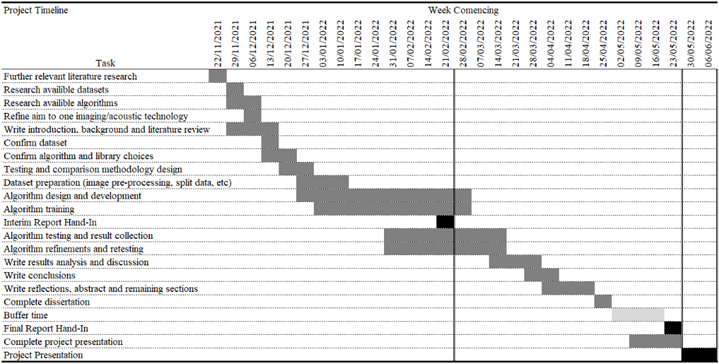
\includegraphics[width=\textwidth]{figures/gantt-chart.png}
    \caption{Project plan presented as a Gantt chart.}
    \label{fig:gantt-chart}
\end{figure}

\subsection{Risks}
During any project, there are always risks that can be encountered and if no mitigation plan is in place, then it can lead to delays in the project. As part of the project management within this project, a full risk assessment was performed and mitigation planned to avoid any lost time. This was integrated into the project management methodology, by allowing for a buffer time within the waterfall plan of the overall project. The risk management table can be seen in \autoref{tbl:risk-table}.

\begin{table}[H]
    \caption{Risks likely to be encountered during this project.}
    \centering
    \begin{tabular}{p{0.22\textwidth}|p{0.11\textwidth}|p{0.14\textwidth}|p{0.41\textwidth}}
    Risk & Impact & Likelihood & Mitigation\\
    \hline\hline
    No availability of suitable training datasets. & High & Medium & While researching which imaging/sound source to use (CT, X-Ray, Acoustic), ensure there is sufficient availability of datasets and dataset size before beginning algorithm development.\\
    Algorithm requires significant computational performance that cannot be supplied. & Medium & Medium & When researching and selecting which machine learning algorithms will be used for evaluation, take note, and ensure that only resource efficient models are used. This will both mitigate the risk for training and testing the algorithms during this project and reflect hardware requirements of real-world use.\\
    Algorithm will not function due to   unavailable libraries or hardware requirements. & Medium & High & When selecting which machine learning algorithms will be used for evaluation, check each algorithm’s prerequisite hardware requirements, and ensure they are open source and available for use by all.\\
    Machine learning techniques or algorithms suddenly becomes closed source and cannot be used. & Medium & Low & Regularly check usage rights of each algorithm and select algorithms open source by nature.\\ 
    \end{tabular}
    \label{tbl:risk-table}
\end{table}

\section{Software Development}
Software development and the Software Development Life Cycle (SDLC) are important to all software products, solutions and research. The SDLC acts as a guide for the planning, development and delivery of any software focused project, in this case the planning of the problem domain, the development of multiple machine learning models and the delivery of evaluated results as a product of this software.

The kanban approach was again used to guide software development, taking the kanban board and sectioning work items into stages of the SDLC: Backlog, Requirements, Design, Development, Testing, Deployment, Done. Put into context, a model not yet developed or researched, would be placed into the backlog, moving into the requirements section as research into existing implementations and dependencies of the model were carried out. When a model was in the design section, the structure of the model (e.g. hidden layer formatting) was put in place. In development the model would be built within a development environment, tested in the testing section and finally evaluated against the dataset when in the deployment section.

Using this methodology when developing software for this project comes with the same advantages as it does for managing the project. Minimising work in progress means that a focus is on delivering working and evaluated models, while continually measuring and improving the life cycle of development for each model. This continual adaptability and flexibility means that kanban is especially suited to this project and serves towards the test and improve nature of it.

\section{Toolsets and Machine Environments}
There are a number of toolsets used within this projects artefact, both software and hardware related. In order to reproduce the artefact, these must be installed as prerequisites to the project.

\subsection{Software Requirements}
The following sections introduce the software used to complete this research project. While some software, like the development environments and visualisation software like TensorBoard are optional and are not needed to train the models, some modification to the code might be needed to run without them.

\phantomsection

\subsubsection{Python}
Python was the chosen language for this project, due to a number for reasons. Firstly Python is the most popular programming language worldwide, with a 27.85 \% market share, according to the PYPL index \citep{PYPLPopu3:online}, seen in \autoref{tbl:PYPL-table}. This means not only is it well known by computer and data scientists, it is also well supported by both its richness of available libraries and its documentation. Its popularity directly influences its choice for project, by allowing others to pick up and further improve on findings from this research. Other languages in the PYPL list, such as Java, JavaScript and C\# also have a large community and wide documentation, however there are still other factors that set Python apart from these, making it the final choice. 

\begin{table}[H]
    \caption{PYPL Worldwide Index, May 2022 \citep{PYPLPopu3:online}.}
    \centering
    \begin{tabular}{c|l|r}
        Rank & Language & Share \\
        \hline\hline
        1 & Python & 27.85\% \\
        2 & Java & 17.86\% \\
        3 & JavaScript & 9.17\% \\
        4 & C\# & 7.62\% \\
        5 & C/C++ & 7.0\% \\
        6 & PHP & 5.36\% \\
        7 & R & 4.34\% \\
        8 & TypeScript & 2.39\% \\
        9 & Objective-C & 2.25\% \\
        10 & Swift & 2.05\% \\
    \end{tabular}
    \label{tbl:PYPL-table}
\end{table}

Python's availability of libraries is also a direct influence of choice for this project, as the majority of machine learning and deep learning libraries are supported by Python, such as TensorFlow, PyTorch and Scikit-Learn, with its dominance expected to remain for the foreseeable future \citep{raschka2020machine}. This is compared to libraries like DeepLearning4j, a deep learning library for Java, which, while comparable to the Python libraries, has a declining use within the medical field \citep{erickson2017toolkits}. 

Finally Python has a very natural syntax which is very close to the English language, making it very readable, even by those with no prior knowledge of the language, compared to the likes of Java and C\# \citep{srinath2017python}.

The entirety of the projects code was written in Python and such is a hard requirement to run the projects artefact. It is recommended to use Python 3.7 or later for TensorFlow support.

\subsubsection{TensorFlow - Keras}
TensorFlow with Keras as the API layer was the chosen machine learning library for this project. TensorFlow is an "end-to-end open source platform for machine learning" with an eager execution environment \citep{TensorFl5:online}. TensorFlow is built upon tensors, which are immutable, multi-dimensional arrays, that are used to store objects, classes and weights that propagate through neural networks. TensorFlow was chosen over other libraries like PyTorch and SciKit-Learn for several reasons, one such reason is due to is eager execution, which means one can view results of operations instantly, as tensors are updated as they are called upon within the code. This allows one to quickly judge the success of a particular model instantly, as it trains, resulting in quick debugging. Another reason for choosing TensorFlow, was its integration with Keras, an API written to run on top of TensorFlow, which makes the creation of machine learning models simple and fast with its sequential model \citep{AboutKer65:online}. The sequential model is a linear stack of layers which allows a user to prototype and build models from scratch, or improve on an existing library of models easily. Keras supplies over 30 pre-trained deep learning models for use within its API, this is a key feature in this project as it allows for accurate replication of the chosen models for evaluation and use of transfer learning in selected models.

TensorFlow and Keras are amongst the most popular machine learning libraries for research studies and business use cases, making both its development support and its applicability in real world use cases beat out competitors. \cite{hale2018deep} ranked each library against each other based on a power score, calculated by the weighted scores of popularity from multiple data sources, seen in \autoref{fig:ml-power-scores}. 

\begin{figure}[H]
    \centering
    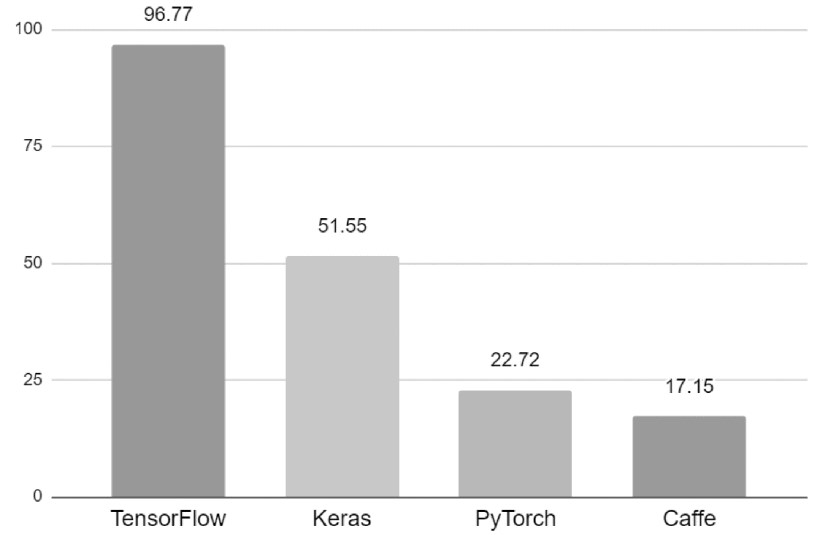
\includegraphics[width=0.65\textwidth]{figures/ml-power-sources.jpg}
    \caption{Power scores of various machine learning libraries \citep{hale2018deep}.}
    \label{fig:ml-power-scores}
\end{figure}

The TensorFlow and Keras are used in the entirety of this project and such is a hard requirement to run the artefact. It is recommended to use TensorFlow 2.0 and Keras 2.0 or later, but with some code modifications, TensorFlow 1.0+ and Keras 1.0+ can also be used.

\subsubsection{TensorBoard}
TensorBoard is a visualisation library for TensorFlow, that tracks and plots metrics from TensorFlow models as they train \citep{TensorBo28:online}. Within this project, TensorBoard was used to both extract visual data of the models performs, like accuracy and loss metrics, as well as tracking weather a particular model was over/under fitting. TensorBoard was chosen over other visualisation libraries like Matplotlib or seaborn due to it's tight integration with TensorFlow, and interactivity. TensorBoard also allows one to implement and track hyper-parameter tuning within a project, this was extremely beneficial for this project.

In this project, TensorBoard 2.8.0 was used and is a hard requirement to run the artefact. As with TensorFlow, it is recommended to use TensorBoard 2.0 or later, but with some code modifications, TensorBoard 1.0+ can also be used.

\subsubsection{Scikit-Learn}
Scikit-Learn is a machine learning library built for Python, which is bundled with many evaluation functions \citep{33Metric9:online} and cross validation functions \citep{31Crossv34:online}. The evaluation functions used within Scikit-Learn provided accuracy, precision, recall, F1 score and confusion matrix metrics, for each trained model in the project. Scikit-Learn's evaluation functions were chosen over Keras' inbuilt functions as Keras' own evaluation functions are limited to only providing loss and accuracy data\citep{Modeltra48:online}, with other metrics having to be calculated manually, making Scikit-Learn a faster and easier to implement solution. 

Scikit-Learn's Stratified K-Fold cross validation implementation was also used within this project. This is used to ensure fairness when evaluating models performance, by taking an average of each folds validation accuracy', the possibility of dataset or training inconsistencies are removed. Keras offers no in built solution to cross validation, so much like the evaluation metrics, has to be performed manually, making Scikit-Learn a faster and easier to implement solution.

Scikit-Learn was also used to shuffle and re-sample the training data, so that there was no bias towards a particular class or model due to possible bias in the dataset structure.

In this project, Scikit-Learn 1.0.2 was used and is a hard requirement to run the artefact.

\subsubsection{Pandas}
Pandas is an open source data manipulation and analysis library for Python \citep{pandasPy63:online}. Pandas was used for loading in the dataset to the artefact, performing some initial pre-processing, like dropping any patient data from the dataset, to remove bloat. Pandas was also used to store and handle the dataset throughout the artefact, using pandas DataFrames, a two dimensional data structure to store tabular data, like the datasets labels.

In this project, pandas 1.3.5 was used and is a hard requirement to run the artefact.

\subsubsection{NumPy}
NumPy is an open source scientific and mathematics library for Python \citep{NumPy90:online}. NumPy was used for basic numerical operations within the project, and is also a dependency for other libraries used. 

In this project, NumPy 1.21.6 was used and is a hard requirement to run the artefact.

\subsubsection{Google Cloud Platform - Development Environment}
Google Cloud Platform was used in this project to train and test the initial selection of the six COVID-19 classification models and perform hyper-parameter tuning on each model. Two services used within Google Cloud Platform were Vertex AI \citep{VertexAI57:online} and Cloud Storage \citep{CloudSto72:online}. Vertex AI enables fast code building though Vertex AI Workbench, a Jupyter notebook environment with access to server grade GPUs. This enabled quick testing and finalisation of the first round of models for evaluation within this project. Vertex AI also has the ability to execute notebook runs on specific hardware and software instances in parallel, meaning fairness though out the first stages of model evaluation and a fast time to results thanks to the allocated NVIDIA Tesla K80s for each instance. Cloud storage was used to store the COVIDx-CXR database the models were trained on, alongside the saved trained model weights and the TensorBoard logs.

Google Cloud Platform and its subsidiary solutions are not a requirement to run the artefact.

\subsubsection{Google Colab - Development Environment}
Google Colaboratory (Colab) is an online Jupyter notebook style Python development environment designed for machine learning and data analysis \citep{GoogleCo52:online}. Colab is equipped with pre-installed data manipulation and machine learning libraries, including all those used in this project, and provides access to fast computing resources like GPUs. This makes developing and executing machine learning experiments, like this project, accessible and fast, with the ability to share to other researchers. This development environment was used for the initial building of all models, and the final evaluation of the best models found. One downside, however, is the fact that computing resources are not guaranteed, meaning that if demand for resources is high, or a notebook has been running for particularly long, then there is a possibility that it might be terminated.  

Google Colab is not a requirement to run the artefact, however a Jupyter notebook solution, like this, must be used.

\subsubsection{GitHub}
GitHub is an online Git version control software offering source code management and internet hosting for projects. In this project GitHub was used as both a version control software and a code hosting tool, to ensure there was a backup of all code, for each version authored, and for seamless transfers between Google Cloud Platform and Google Colab.

GitHub is not a requirement to run the artefact, however can been used to access the project files.

\subsection{Hardware Requirements}
While TensorFlow can run on a large number of devices, there are some hardware limitations, especially if a Graphical Processing Unit (GPU) is used to accelerate performance. TensorFlow requires a CPU capable of AVX instructions, which most modern Computational Processing Unit's (CPU) support \citep{InstallT17:online}. If GPU acceleration is required and the device used has an NVIDIA GPU, then it must support compute unified device architecture (CUDA), a "parallel computing platform" which can "dramatically speed up computing applications by harnessing the power of GPUs" \citep{CUDAZone2:online}. If the device has a GPU that does not support CUDA, but does support DirectX 12 (e.g. an AMD GPU manufactured in the last several years), then Microsoft's DirectML can be used enable GPU support for TensorFlow \citep{Introduc93:online}. Precautions must be taken if DirectML is used however, as it has differing version requirements of Python, TensorFlow and NumPy.

\section{Research Methods}
In order to to gather and analyse data collected to evaluate the selected models of this project, a few different research method were carried out and particular testing structures were set in place.

Firstly, the structure in which to gather the primary quantitative data was devised, this ensured an unbiased and fair standard was followed for each model. The structure is detailed throughout the following sections.

\subsubsection{Initial Training}
All six models were optimised using hyper-parameter tuning using a Google Cloud Platform Vertex AI parallel notebook execution process. This was performed on a small portion of the COVIDx-CXR dataset, meaning that the training time for larger models did not exceed the allotted time for this stage of the project and allotted hardware resources within Google Cloud Platform were not depleted. All models were trained with the same batch size of 32, the same image resolution of 224 x 224





You should investigate the types of research methods necessary to validly answer the research questions that your project addresses. You should cite relevant sources to justify your choices.
\begin{itemize}
    \item abductive
    \item primary data
    
\end{itemize}

% Design, Development and Evaluation
\chapter{Design, Development and Evaluation}
\section{Project Requirements}
\subsection{Software Requirements}
In order to reproduce the artefact, software requirements must be installed and hardware requirements must be met as prerequisites to the project. While some software, like the development environments are optional and are not needed to train the models, some modification to the code might be needed to run without them.

\phantomsection
\subsubsection{Python}
The entirety of the projects code was written in Python and such is a hard requirement to run the projects artefact. It is recommended to use Python 3.7 or later for TensorFlow support.

\subsubsection{TensorFlow and Keras}
The TensorFlow and Keras are used in the entirety of this project and such is a hard requirement to run the artefact. It is recommended to use TensorFlow 2.0 and Keras 2.0 or later, but with some code modifications, TensorFlow 1.0+ and Keras 1.0+ can also be used.

\subsubsection{TensorBoard}
In this project, TensorBoard 2.8.0 was used and is a hard requirement to run the artefact. As with TensorFlow, it is recommended to use TensorBoard 2.0 or later, but with some code modifications, TensorBoard 1.0+ can also be used.

\subsubsection{Scikit-Learn}
In this project, Scikit-Learn 1.0.2 was used and is a hard requirement to run the artefact.

\subsubsection{pandas}
In this project, pandas 1.3.5 was used and is a hard requirement to run the artefact.

\subsubsection{NumPy}
In this project, NumPy 1.21.6 was used and is a hard requirement to run the artefact.

\subsubsection{Google Cloud Platform - Development Environment}
Google Cloud Platform and its subsidiary solutions are not a requirement to run the artefact, however can be used to run model training simultaneously.

\subsubsection{Google Colab - Development Environment}
Google Colab is not a requirement to run the artefact, however a Jupyter notebook solution, like this, must be used.

\subsubsection{Project Code}
The project code is hosted on GitHub, and can be accessed and downloaded through the following link: \url{https://github.com/laurencebrwn/ml-covid19-eval}. The results and individual models notebook files are all found here.

\subsubsection{COVIDx-CXR Dataset}
The dataset used to train the image classification models is a hard requirement for this project. The full dataset is hosted on kaggle, and can be found here: \url{https://github.com/lindawangg/COVID-Net/blob/master/docs/COVIDx.md}. The images should be obtained from the "COVIDx CXR-2 Kaggle Dataset" link (\url{https://www.kaggle.com/datasets/andyczhao/covidx-cxr2}) detailed on the previously linked page. The labels for both binary ("train\_COVIDx9B.txt" and "test\_COVIDx9B.txt") and multi-label ("train\_COVIDx9A.txt" and "test\_COVIDx9A.txt") classification, can be downloaded from the link (\url{https://github.com/lindawangg/COVID-Net/tree/master/labels}) detailed on the previously linked page.

\subsection{Hardware Requirements}
While TensorFlow can run on a large number of devices, there are some hardware limitations, especially if a Graphical Processing Unit (GPU) is used to accelerate performance. TensorFlow requires a CPU capable of AVX instructions, which most modern Computational Processing Unit's (CPU) support \citep{InstallT17:online}. If GPU acceleration is required and the device used has an NVIDIA GPU, then it must support compute unified device architecture (CUDA), a "parallel computing platform" which can "dramatically speed up computing applications by harnessing the power of GPUs" \citep{CUDAZone2:online}. If the device has a GPU that does not support CUDA, but does support DirectX 12 (e.g. an AMD GPU manufactured in the last several years), then Microsoft's DirectML can be used enable GPU support for TensorFlow \citep{Introduc93:online}. Precautions must be taken if DirectML is used however, as it has differing version requirements of Python, TensorFlow and NumPy.

\section{Design}
In order to design the software that would train and evaluate each of the selected models, identified in the literature review, prompts were taken from the methodology to devise a structure that would form each models notebook. By implementing a general structure that all models would inherit, it made changes to the models, hyper parameters easy, while reducing development time. While there are a few variations for each model a common format was followed for all models:

\begin{enumerate}
    \item Set up the environment.
    \begin{enumerate}
        \item Define the model and training variables.
        \item Import the required libraries, like TensorFlow, Keras, Scikit-Learn, etc.
        \item Define the hyper-parameters of the model (or list of hyper-parameters if performing tuning).
    \end{enumerate}
    \item Prepare the dataset.
    \begin{enumerate}
        \item Read in the label files for both test and train.
        \item Down-sample each class to match the total dataset size and to ensure all classes are equally represented.
        \item Shuffle the data.
        \item Pre-process the X-Ray images (and perform image transformations on the training dataset).
        \item Split the training data into folds for stratified K fold cross validation.
    \end{enumerate}
    \item Create the machine learning model.
    \begin{enumerate}
        \item Create the Keras sequential model.
        \item If the model is using transfer learning (Xception, ResNet and DenseNet), fetch the base model from Keras' application library.
        \item Define the model layers in the sequential model.
        \item Set any hyper-parameters, like the optimiser, learning rate etc.
        \item Compile the model.
    \end{enumerate}
    \item Begin cross validation training.
    \begin{enumerate}
        \item Iterate through hyper-parameter variations.
        \item Iterate through stratified K folds.
        \item Train the model.
        \item Record model logs.
        \item Save the model weights.
    \end{enumerate}
    \item Evaluate the model.
    \begin{enumerate}
        \item Iterate through the trained models.
        \item Load model weights.
        \item Predict the labels on the test dataset.
        \item Record the models key metrics, described in the methodology.
        \item Save the models metrics and performance
    \end{enumerate}
\end{enumerate}

\section{Developing the Artefact}
Developing the Python notebooks for each model followed a similar flow to that listed in the design section. Firstly the Environment set up was developed, followed by dataset preparation and pre-processing. Where the development flow differed was that the cross validation training and evaluation sections were developed before the model itself. This meant a skeletal structure consisting of everything except for the model itself could be replicated, once for each model. This section will detail the development via a run through of the code itself, split into the sections listed in the flow above.

\subsection{Environment Set Up}
Firstly the correct environment had to be set up before any machine learning models were created or training was to happen. This started with defining the image size, batch size, dataset size, number of K folds, the maximum amount of epochs and the path to the dataset. Secondly all the required libraries were imported. This included NumPy, pandas, TensorFlow, Scikit-Learn, TensorBoard and other generic Python libraries like those used to record the time. Finally the hyper-parameters were instantiated. This was done using TensorBoard's "hparams" plugin. An example of this can be seen in \autoref{fig:hyper-param-code}.

\begin{figure}[H]
    \centering
    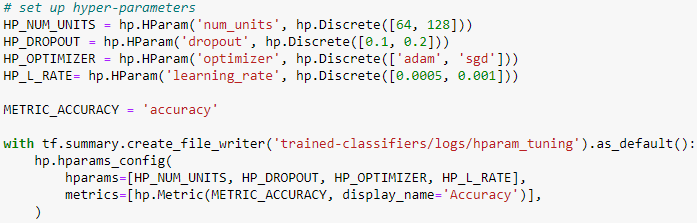
\includegraphics[width=\textwidth]{figures/hyper-param-code.png}
    \caption{Defining the hyper-parameters with TensorBoard.}
    \label{fig:hyper-param-code}
\end{figure}

\subsection{Dataset Preparation}
Next the COVIDx-CXR dataset had to be brought in, and manipulated such that the models could use it for training. To begin, the dataset labels were read in, and unnecessary columns, like "patient id" and "data source" were removed. Next the data was down-sampled, such that the classes were of equal proportions, and thoroughly shuffled. This was done with Scikit-Learns "resample" function, an example of this can be seen in \autoref{fig:dataset-downsampling}. 

\begin{figure}[H]
    \centering
    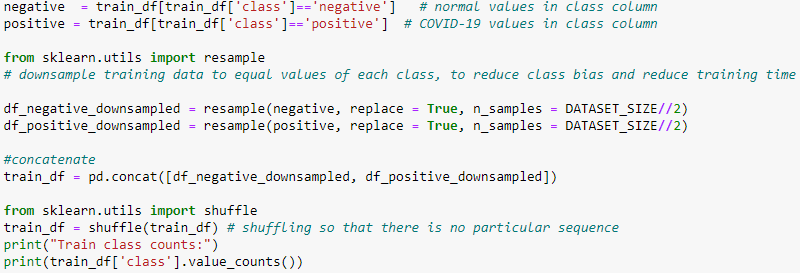
\includegraphics[width=\textwidth]{figures/dataset-downsampling.png}
    \caption{Down-sampling and shuffling the dataset.}
    \label{fig:dataset-downsampling}
\end{figure}

The dataset labels then had to be linked with the corresponding images. This was done with Keras' "ImageDataGenerator". Using "ImageDataGenerator" allowed for the use of the "flow\_from\_dataframe()" function, which matches up the image paths, stored in a DataFrame, to the images themselves. It also allowed for image pre-processing to be performed serially, each time an image was flowed from the DataFrame. While the image pre-processing remained mostly constant for each model, some models, like Xception, ResNet and DenseNet, each had a specific pre-processing, created for that model, by Keras. Pre-processing the training images also took a different form from the test images, as the data had to be split into training and validation folds, dictated by the stratified K fold implementation. A separate function was made for this purpose, an example of which, used for the Xception model, can be seen in \autoref{fig:image-preprocessing}.

\begin{figure}[H]
    \centering
    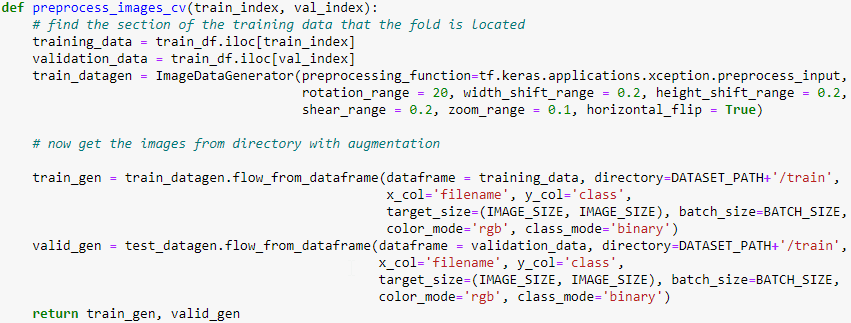
\includegraphics[width=\textwidth]{figures/image-preprocessing.png}
    \caption{Down-sampling and shuffling the dataset.}
    \label{fig:image-preprocessing}
\end{figure}

\subsection{Creating the Models}
Next each of the six models had to be built, while each models architectures differ, each model uses some or all of the same layers. To understand this better some research was carried out on each layers functions. The following is an explanation for layers used in the models:

\begin{itemize}
    \item Dense -  A deeply connected neural network layer (all neurons receive inputs from all neurons in the previous layer) performs matrix-vector multiplication, with the values of said matrix being trained and updated with back propagation \citep{Denselay11:online}.
    \item Conv2D - Creates a convolution kernel that is convolved with the input, in this case an image, or the previous layers output. The result of the kernel produces a tensor of outputs \citep{Conv2Dla69:online}.
    \item GlovalAveragePooling2D - Down-samples the entire feature map to a single value. In a 2D layer it takes a 4D tensor and returns a 2D tensor with the shape of (batch size, number of channels) \citep{GlobalAv91:online}.
    \item BatchNormalization - Normalises its inputs by applying a transformation that maintains the outputs mean to as close to 0 as possible and its standard deviation as close to 1 as possible \citep{BatchNor52:online}.
    \item Dropout - Randomly sets inputs values to 0, at a user defined frequency, to prevent over fitting. Those inputs that are not set to - are scaled so that the total sum of the inputs is unchanged \citep{Dropoutl66:online}.
    \item Activation - Applies a user defined activation function to the input, while retaining the input shape \citep{Activati33:online}.
    \item MaxPooling2D - Similar to GlobalAveragePooling 2D, in that it down-samples the entire feature map, but this time takes the maximum value over a user defined input window, known as a pool size \citep{MaxPooli1:online}.
    \item Flatten - Flattens the input to a 1D shape, while retaining the batch size \citep{Flattenl52:online}.
\end{itemize}

The models were created inside a create\_model() function which takes the hyper-parameters as an input, and returns the model as an output. Inside the function the Keras sequential or functional API is used to create the model, before defining its optimiser and learning rate, before compiling the model. An example of this, used for the Xception model can be seen in \autoref{fig:xception}.

\begin{figure}[H]
    \centering
    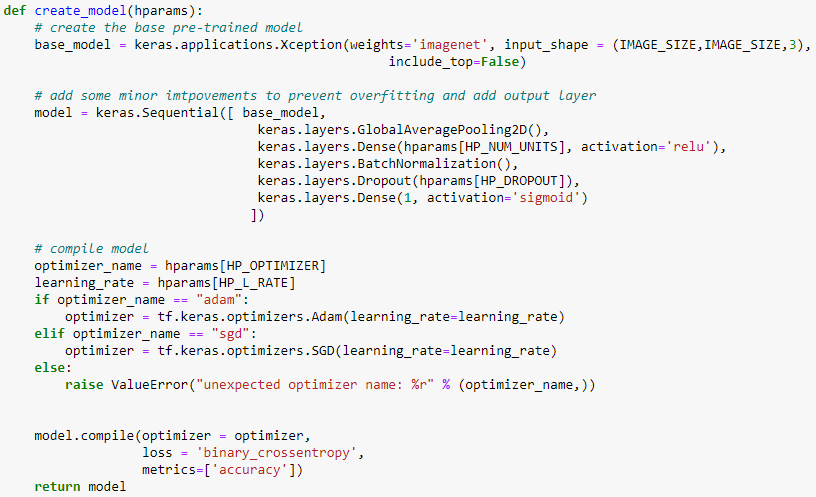
\includegraphics[width=\textwidth]{figures/xception.png}
    \caption{The create\_model() function structure, used for creating Xception in this case.}
    \label{fig:xception}
\end{figure}

While model architecture of the used models are standard, each model has been slightly modified initially for better performance, and to match the correct output specification (ie. number of classes). Each model has a different architecture and layer structure, and the following sections will explain in detail the model architecture for each, including any modifications made.

\phantomsection
\subsubsection{AlexNet}
Since Keras has no application model available for AlexNet, it had to be reproduced manually using Keras' sequential API. A description of the architecture, taken from \citep{krizhevsky2012imagenet}, was used for this.

AlexNet consists of 5 Conv2D layers, each of which is followed by a BatchNormalization layer, an Activation layer with a rectified linear activation function (ReLU) and a MaxPooling2D layer, before being passed to the next Conv2D layer. Following this the output is flattened, and passed to 3 Dense layers, each of which is followed by a BatchNormalization layer, an Activation layer with a rectified linear activation function (ReLU) and a Dropout layer. This is finally followed by an output layer, which is a Dense layer with a single output (for binary classification), a BatchNormalization layer and an Activation layer with a sigmoid activation function.

Hyper-parameter tuning involved changing the final Dense layers number of units, all three dense layers dropout values, the optimiser and the learning rate. The full model code can be seen in \autoref{fig:alexnet-part1} and \autoref{fig:alexnet-part2}.

\subsubsection{DenseNet201}


\subsubsection{ResNet50V2}


\subsubsection{SqueezeNet}


\subsubsection{Xception}


\subsubsection{ConvNet}


\subsection{Cross Validation Training}


\subsection{Model Evaluation}


\section{Operation of Artefact}

\section{Initial Results}

\section{Model Improvements}

\section{Final Results}


% Conclusions
\chapter{Conclusions}
This study set out to analyse of the effectiveness of multiple machine learning algorithms to establish the best suited at diagnosing COVID-19. Throughout numerous trials and comparisons almost 100 models of varying configurations were tested. From the analysis of the results in the previous section the model best suited at diagnosing COVID-19 is the Xception network which made use of transfer learning from the ImageNet weights. Modifications to the network that proved the strongest were the addition of a GlobalAveragePooling2D layer that received Xception’s output, followed by a Dense layer with a rectified linear activation function (ReLU), followed by a BatchNormalization layer and a Dropout layer. The hyper-parameters that functioned best with this modified network were 128 Dense units, a dropout of 0.1, the Adam optimiser and Learning rate of 0.001. For the sake of this conclusion this specific model and configuration will be referred to as XceptionCov19. The full model diagram of XceptionCov19 can be seen in \autoref{fig:xceptioncov19}.

Comparing these results to other studies identified within the literature review, the best model identified in this study has differing results. Comparing firstly with \cite{zhang2020covid19xraynet} COVID19XrayNet model which produced an accuracy of 0.9192 when trained on a multi-label classification dataset, the XceptionCov19 model built in this study outperforms it by a large margin. When XceptionCov19 was trained on a small multi-label classification dataset it produced an accuracy result of 0.9335, and a result of 0.9530 when trained on a large multi-label classification dataset. Using metrics from the large multi-label classification dataset training, XceptionCov19 improves on COVID19XrayNet's performance by 0.0338, a 3.7\% increase in accuracy. COVID19XrayNet only trained on two databases that combined to a total of 6,195 images however, even when XceptionCov19 trained on a smaller dataset of 1,500 images it still produced a better result.

Comparing the results of XceptionCov19 against those of \cite{fitriasari2021improvement} Xception and ResNet inspired model, the multi-label classification results are closer. When \cite{fitriasari2021improvement} model trained on a total of 1,398 images of 4 classes, compared to XceptionCov19's 3 multi-label classes, it produced accuracy results of 0.9341, a marginal improvement over XceptionCov19's 0.9335 when trained on the small multi-label classification dataset, but not as strong as XceptionCov19's accuracy of 0.9530 when trained on a large multi-label classification dataset.

The \cite{bressem2020comparing} study compared many different models, much like this study, and its best performing model was DenseNet201. This model produced a pooled AU-ROC score of 0.998 when training on a 3 class multi-label dataset of 46,754 images. While the study does not provide accuracy results to compare with, AU-ROC scores were calculated separately for this comparison. The AU-ROC graphs for XceptionCov19 can be seen in \autoref{fig:au-roc-all}. XceptionCov19's mean AU-ROC score across its five folds is 0.962 when performing multi-label classification on the large dataset. While \cite{bressem2020comparing} DensNet201 did perform better, the model was also pre-trained on the CheXpert dataset (a collection of over 200,000 chest X-Ray images), which is likely to have improved DenseNet201's performance significantly.

With these findings it is clear that XceptionCov19 is at the forefront of COVID-19 classification, sharing similar and in some cases improved results over other state-of-the art models currently developed. XceptionCov19's accuracy percentage is 97.80\%, this is far above the 71.4\% accuracy of doctors' clinical vignettes diagnoses tests \citep{richens2020improving}. XceptionCov19's AU-ROC score is also higher than those of PCR tests, with 0.962 versus 0.879 respectively \citep{mardani2020laboratory}.

The performance of XceptionCov19 could be further improved in the future when larger and more diverse datasets become available. If computing power availability and time was not an issue more improvements could also be made if XceptionCov19 was pre-trained on a medicinal dataset, such as CheXpert. 

To conclude the XceptionCov19 model is among the best in the current space of COVID-19 classification models at diagnosing COVID-19 cases. It should be able to successfully support a doctor's diagnoses by providing a second opinion if implemented as an automatic diagnoses tool within hospitals.

% Reflective Analysis
\chapter{Reflective Analysis}
This section aims to give a critical reflection of my own thoughts on the project. While many aspects of the project went well, some could have been improved if undertaken again. To aid in this analysis,segments of the Gibbs reflective cycle were used to help structure this section \citep{gibbs1988learning}.

\section{Positive Aspects of the Project}
Many aspects of this project were positive, the first of which is the development of the artefact itself. Throughout the duration of this project I built a solid framework in which to train and evaluate many models and variations quickly and efficiently. When beginning the project I dedicated a lot of time to learning the various libraries involved and methods that other researchers used to carry out such evaluations, this helped significantly in building this robust artefact. The artefact can be used in the future if necessary, for further evaluations in this space or to re-apply in other projects.

Another aspect of this project that went well was the model performance itself. My expectations going into this project were that it would be unachievable to build a model as successful as other published papers. The results of the best models in the study speak for themselves and with the excellent performance metrics of the final model, I feel very accomplished having even beaten other studies model performance. This is not to say that the model performances achieved in this study are unrivalled or ground breaking, but being able to judge my results on par with others results was a success in itself.

I was also able to gain a deep understanding of machine learning, deep learning and the toolsets required to enable these. Learning the workings of libraries like Keras and TensorFlow has served me well for not only this project, but will help me in the future by being able to apply this knowledge to the industry. It also enabled me to quickly recreate other researchers models from architecture diagrams, like \cite{fitriasari2021improvement} Xception-ResNet model. Using Google Cloud Platform as a development environment was a particularly beneficial part to this project, as it saved days worth of training time by enabling me to train models in parallel, by splitting execution tasks among many virtual servers.

Finally the analysis of the models went smoothly, by devising the entire project plan I would use beforehand within the methodology and applying this in my evaluation allowed me to quickly judge and compare models in this study and others critically. 

\section{Negative Aspects of the Project}
While a lot of the project went well there were some items that did not. Inconsistencies of metric recording is one example. While I had a methodology in place of which metrics I would use to evaluate the performance, there were some discrepancies on where that data came from. It is accepted that model performance can be taken from the mean results of cross validation on the validation dataset or the best performance on the test dataset from the folds used in cross validation. During the first round of model testing I had not known this, so the initial models were judged by their mean scores on each five folds performance on the test dataset. Following on from this I made sure to record all validation and test data for each fold individually. I used this for reference, but the mean test metrics were still used as the main metric. Other studies, for example \cite{bressem2020comparing}, also used a similar format of metric recording so I was still able to draw comparisons however. By using a uniform method to record every metric from each fold, this would not have been much of an issue.

Another portion of the project that did not go as intended was the model improvements. While I managed to learn about what modifications did not work well and what modifications reduced training time, I was not able to improve Xception's performance beyond the original modifications I had made. Perhaps it might have been better to evaluate all of the models in the initial round with no modifications whatsoever, except those required to fit the dataset image size and number of classes. Then I could have used my initial modification within the improvements round, and worked off of that instead. Another thing that might have helped resolve this was to explore more literature during the first phase of the project that focused on machine learning and deep learning network modification for performance. I could have then taken this onto the model improvements round and tested any theories I might have come up with from literature research.

The final major negative aspect is one that was beyond control, but identified within section \ref{risks}, was the need for significant computational performance for larger algorithms. While the models selected were efficient when discussed in literature, for example \cite{KerasApp92:online}, I did not take into account the time taken for hyper-parameter tuning and the size of the COVIDx-CXR dataset. While I performed some mitigation to reduce over-running on time during the project for training, it still took longer than I had hoped. I was able to use a reduced sample of COVIDx-CXR, as I reffered to as the "small dataset", this reduced training time during initial rounds. I was also able to use Google Cloud Platform to train models in parrallel, which again reduced time for training. The fact that each model had to train against a dataset five times for cross validation, multiplied by the number of hyper-parameter configurations for each network, it still took a significant amount of time. In the end I depleted the "free \$300 trial credits" within Google Cloud Platform right after initial training. This meant I had to rely on Google Colab for the remainder of the project, which had a limited run time of 12 hours per notebook. Fortunately the longest training time of the models (Xception - Original Improvements, on the large dataset) ran for just under this amount of time. In hindsight, I could have secured funding or planned computational requirements beforehand to reduce the chance of over-running on time for this section of the project.

\section{Improvements That Could Have Been Made}
There were several items in this project that had not been performed due to time constraints of the project, that if there had not been constraints I would have performed. The first of which is drawing further inspiration from other COVID-19 classification models. While I did do this during the end of the improvements phase, using \cite{fitriasari2021improvement} Xcpetion-ResNet model, I feel as though more improvements could have been made had I had the time to further research COVID-19 classification studies and recreate others models for myself. As well as aiding in improvements it would also allow me to evaluate performance of other studies models on the same dataset, adding an extra layer of fairness to the project.

Additionally, trialling use of other pre-training methods like the \cite{bressem2020comparing} use of the CheXpert dataset to pre-train models before training on a COVID-19 dataset. Doing this would likely have further improved all models results. I could have also compared the effect of using pre-training methods like these versus no pre-training more directly, instead of assigning a group of networks to make use of pre-training and a group to not.

I would have also liked to have broken down into the Xception model itself and altered the networks layers to trail performance improvements, instead of just appending various layers. This would have given me the opportunity to learn more about the inner workings of the top models and figure out why they were so successful. It would have also possibly yielded better performance improvements over just appending additional layers.

Finally, if I had more time I would have liked to explore the method devised by \cite{kamimura2019neural} to transform the networks tested in this project from multilayered neural networks to ones without any hidden layers. By doing so I would not only gain an understanding of the layout and inner workings of the model itself, I would have been able to interpret the relation between the models input and outputs. This would have essentially allowed me to diagnose how the model classified an image and which segments or features of an image it paid close attention to come to its outcome. By doing this I would be able to ensure the model was picking up on the areas within the X-Rays that medical experts use to diagnose COVID-19, rather than items in an X-Ray that might be typical to a patient with COVID-19 (respirator, etc.).


% end of thesis body
% --------------------------

% Print out the references
\printReferences

% If you want to put some text before the list of games,
% then you can use the following code:
%\begin{ludography}[Ludography / Optional Title]
    %Here are some games.
%\end{ludography}

\appendix
\chapter{AlexNet Design and Results}
\begin{figure}[H]
    \centering
    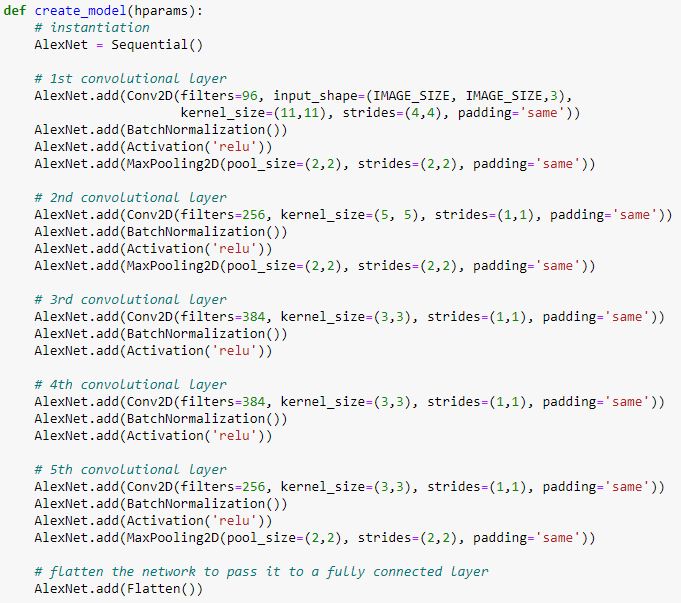
\includegraphics[width=\textwidth]{figures/alexnet-model-part1.png}
    \caption{The 5 Conv2D layers in AlexNet.}
    \label{fig:alexnet-model-part1}
\end{figure}
\begin{figure}[H]
    \centering
    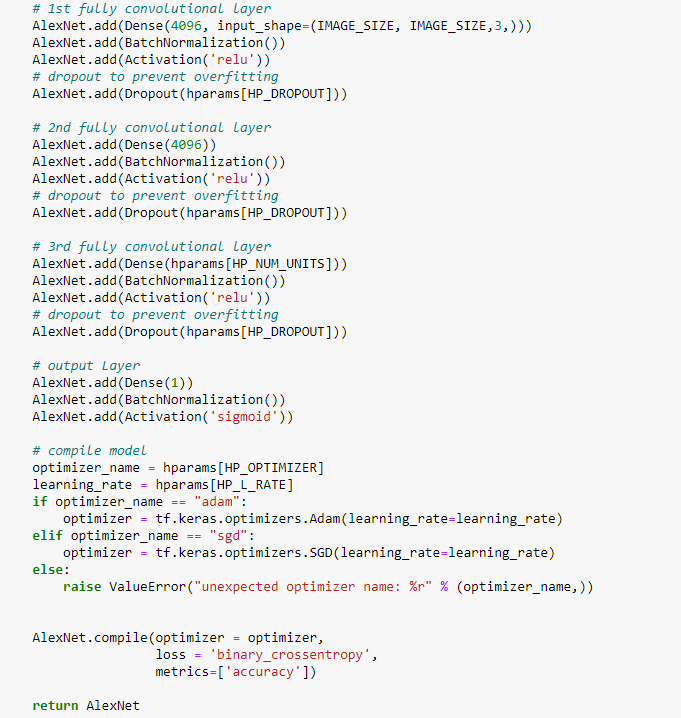
\includegraphics[width=\textwidth]{figures/alexnet-model-part2.png}
    \caption{The 3 Dense layers and output layer in AlexNet.}
    \label{fig:alexnet-model-part2}
\end{figure}

\begin{landscape}
\begin{table}
    \caption{AlexNet results after initial training on the small COVIDx-CXR dataset.}
    \centering
    \begin{tabular}{l|l|l|l|l|l|l|l|l|l}
    Model & Dense Units & Dropout & Optimiser & Learning Rate & \begin{tabular}[c]{@{}l@{}}Mean Test\\ Accuracy\end{tabular} & \begin{tabular}[c]{@{}l@{}}Mean Test\\Precision\end{tabular} & \begin{tabular}[c]{@{}l@{}}Mean Test\\Recall\end{tabular} & \begin{tabular}[c]{@{}l@{}}Mean Test\\F1 Score\end{tabular} & \begin{tabular}[c]{@{}l@{}}Training\\ Time (s)\end{tabular} \\
    \hline\hline
    AlexNet & 1024 & 0.2 & SGD & 0.0010 & 0.7095 & 0.8123 & 0.5480 & 0.6532 & 735 \\
    AlexNet & 1024 & 0.4 & Adam & 0.0010 & 0.6985 & 0.8324 & 0.5400 & 0.6440 & 533 \\
    AlexNet & 512 & 0.2 & SGD & 0.0010 & 0.6895 & 0.8372 & 0.4710 & 0.6017 & 720 \\
    AlexNet & 512 & 0.2 & Adam & 0.0005 & 0.6530 & 0.7341 & 0.5040 & 0.5428 & 495 \\
    AlexNet & 512 & 0.2 & Adam & 0.0010 & 0.6430 & 0.7652 & 0.4220 & 0.5330 & 537 \\
    AlexNet & 1024 & 0.2 & SGD & 0.0005 & 0.6415 & 0.7530 & 0.4350 & 0.5394 & 702 \\
    AlexNet & 512 & 0.2 & SGD & 0.0005 & 0.6380 & 0.7470 & 0.4210 & 0.5326 & 695 \\
    AlexNet & 1024 & 0.4 & Adam & 0.0005 & 0.6350 & 0.6732 & 0.4890 & 0.5635 & 503 \\
    AlexNet & 512 & 0.4 & Adam & 0.0010 & 0.6260 & 0.6266 & 0.4990 & 0.5392 & 509 \\
    AlexNet & 1024 & 0.4 & SGD & 0.0010 & 0.6205 & 0.6875 & 0.4570 & 0.5439 & 679 \\
    AlexNet & 1024 & 0.2 & Adam & 0.0005 & 0.6040 & 0.7090 & 0.3860 & 0.4831 & 437 \\
    AlexNet & 512 & 0.4 & SGD & 0.0010 & 0.6035 & 0.6575 & 0.4350 & 0.5199 & 710 \\
    AlexNet & 1024 & 0.2 & Adam & 0.0010 & 0.6015 & 0.6796 & 0.3740 & 0.4668 & 401 \\
    AlexNet & 512 & 0.4 & SGD & 0.0005 & 0.5855 & 0.6224 & 0.4440 & 0.5143 & 691 \\
    AlexNet & 1024 & 0.4 & SGD & 0.0005 & 0.5655 & 0.5750 & 0.4880 & 0.5256 & 701 \\
    AlexNet & 512 & 0.4 & Adam & 0.0005 & 0.5435 & 0.5310 & 0.4000 & 0.4429 & 366
    \end{tabular}
    \label{fig:alexnet-results}
\end{table}
\end{landscape}
\chapter{DenseNet201 Design and Results}
\begin{figure}[H]
    \centering
    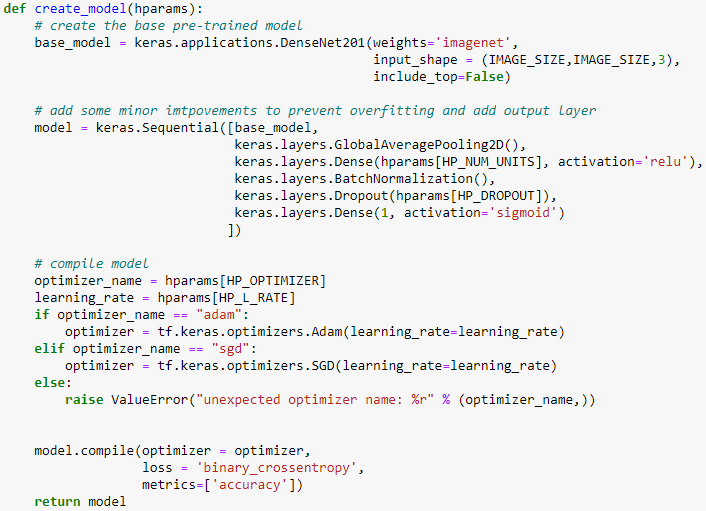
\includegraphics[width=\textwidth]{figures/densenet-model.png}
    \caption{The DenseNet201 model.}
    \label{fig:densenet-model}
\end{figure}
\chapter{ResNet50V2 Design and Results}
\begin{figure}[H]
    \centering
    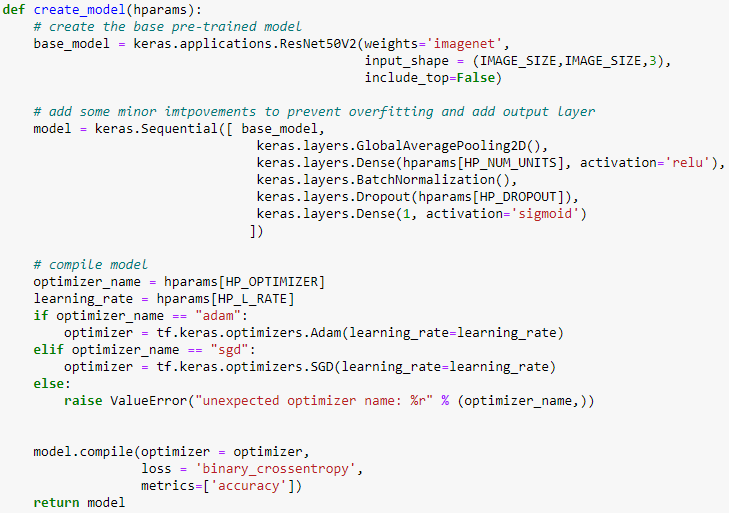
\includegraphics[width=\textwidth]{figures/resnet-model.png}
    \caption{The ResNet50V2 model.}
    \label{fig:resnet-model}
\end{figure}
\chapter{SqueezeNet Design and Results}
\begin{figure}[H]
    \centering
    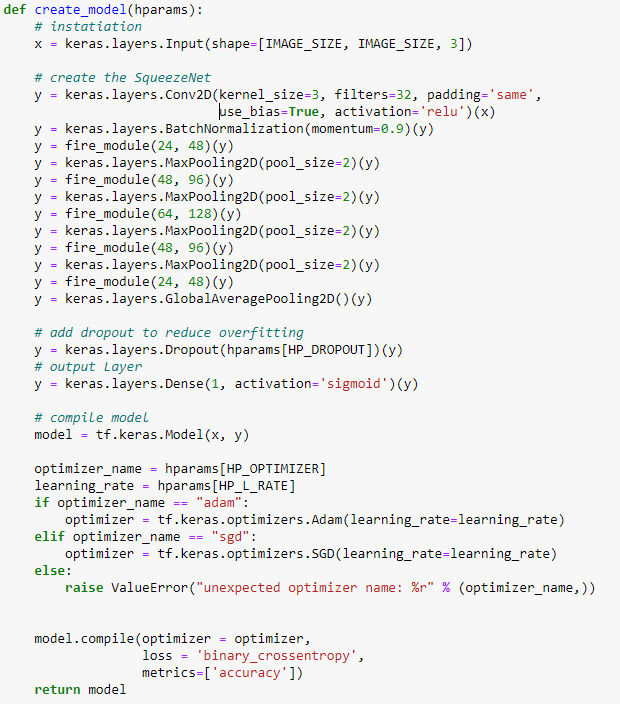
\includegraphics[width=\textwidth]{figures/squeezenet-model.png}
    \caption{The SqueezeNet model.}
    \label{fig:squeezenet-model}
\end{figure}
\begin{figure}[H]
    \centering
    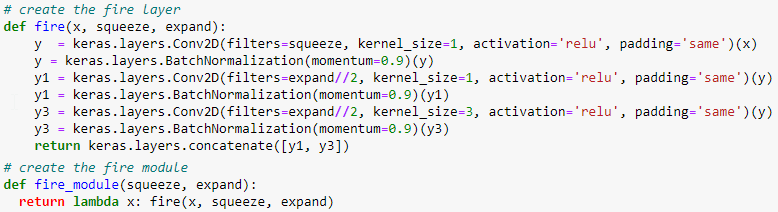
\includegraphics[width=\textwidth]{figures/squeezenet-fire-module.png}
    \caption{The fire module used in the SqueezeNet model.}
    \label{fig:squeezenet-fire-module}
\end{figure}


\begin{landscape}
\begin{table}
    \caption{SqueezeNet results after initial training on the small COVIDx-CXR dataset.}
    \centering
    \begin{tabular}{l|l|l|l|l|l|l|l|l}
    Model &  Dropout & Optimiser & Learning Rate & \begin{tabular}[c]{@{}l@{}}Mean Test\\ Accuracy\end{tabular} & \begin{tabular}[c]{@{}l@{}}Mean Test\\Precision\end{tabular} & \begin{tabular}[c]{@{}l@{}}Mean Test\\Recall\end{tabular} & \begin{tabular}[c]{@{}l@{}}Mean Test\\F1 Score\end{tabular} & \begin{tabular}[c]{@{}l@{}}Training\\ Time (s)\end{tabular} \\
    \hline\hline
    SqueezeNet & 0.2 & Adam & 0.0005 & 0.9290 & 0.9036 & 0.9620 & 0.9316 & 282 \\
    SqueezeNet & 0.1 & Adam & 0.0005 & 0.9165 & 0.8744 & 0.9750 & 0.9213 & 327 \\
    SqueezeNet & 0.2 & Adam & 0.0010 & 0.8980 & 0.9015 & 0.8980 & 0.8911 & 261 \\
    SqueezeNet & 0.1 & Adam & 0.0010 & 0.8965 & 0.8617 & 0.9530 & 0.9027 & 399 \\
    SqueezeNet & 0.1 & SGD & 0.0010 & 0.8275 & 0.7992 & 0.8860 & 0.8351 & 620 \\
    SqueezeNet & 0.1 & SGD & 0.0005 & 0.7815 & 0.7257 & 0.9060 & 0.8045 & 542 \\
    SqueezeNet & 0.2 & SGD & 0.0010 & 0.7710 & 0.7625 & 0.8370 & 0.7857 & 406 \\
    SqueezeNet & 0.2 & SGD & 0.0005 & 0.7650 & 0.7382 & 0.8430 & 0.7825 & 513
    \end{tabular}
    \label{fig:squeezenet-results}
\end{table}
\end{landscape}
\chapter{Xception Design and Results}
\begin{figure}[H]
    \centering
    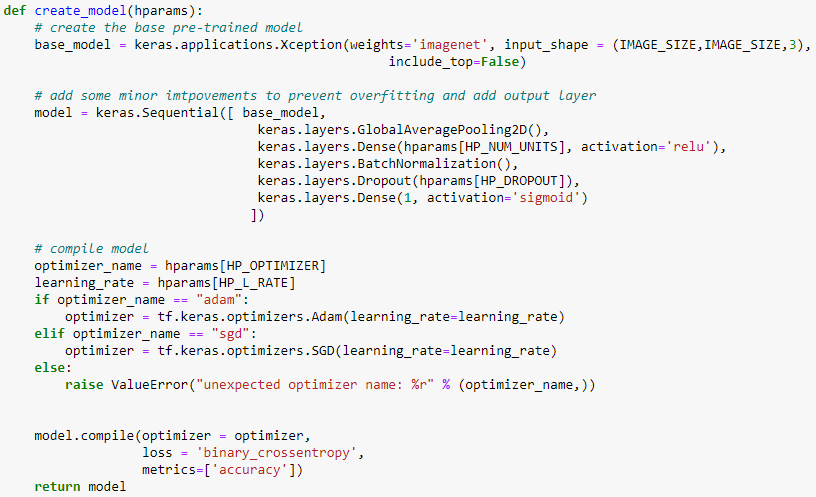
\includegraphics[width=\textwidth]{figures/xception-model.png}
    \caption{The Xception model.}
    \label{fig:xception-model}
\end{figure}
\chapter{ConvNet Design and Results}
\begin{figure}[H]
    \centering
    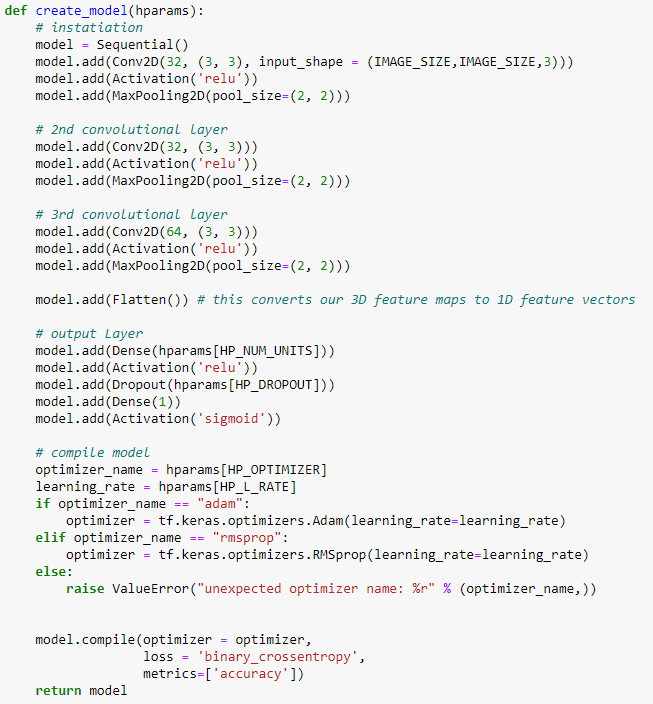
\includegraphics[width=\textwidth]{figures/convnet-model.png}
    \caption{The ConvNet model.}
    \label{fig:convnet-model}
\end{figure}
\end{document}
